\documentclass[b,k,td]{D:/Dropbox/enseignement/CPGE/raphaelpoiree/classe/classe_kara}
\begin{document}
\newcommand*{\classe}{PTSI}
\newcommand*{\partie}{Modèles}
\newcommand*{\titre}{Modèle de TD}
\newcommand*{\numero}{-1}
\newpage
%%%%%%%%%%%%%%%%%%%%%%%%%%%% VERSION ARTICLE %%%%%%%%%%%%%%%%%%%%%%%%%%%%%%%%%%%
\ifthenelse{\boolean{Cours}}{

\mode<article>{
\thispagestyle{empty}
\vspace{0.2cm}

\begin{center}

\rule{\linewidth}{5pt}\\
\begin{minipage}{0.1\linewidth}
\begin{center}
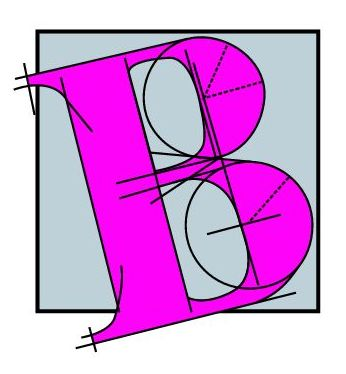
\includegraphics[width=\textwidth]{D:/Dropbox/enseignement/CPGE/raphaelpoiree/paquets/logoBaggio.jpg}
\end{center}
\end{minipage}
\begin{minipage}{0.8\linewidth}
\begin{center}
\vspace{0.2cm}

\large{\MakeUppercase{\partie}}\\

\vspace{0.2cm}

\huge{
Cours \numero \ - \titre
}
\end{center}
\end{minipage}
\begin{minipage}{0.1\linewidth}
\end{minipage}

\vspace{0.4cm}
\rule{\linewidth}{5pt}

\end{center}

\begin{center}
\MakeUppercase{\etablissement} - \MakeUppercase{\auteur} - \MakeUppercase{\classe} - \MakeUppercase{\annee}
\end{center}

\tableofcontents
%\minitoc

%\vfill

%\vspace{1cm}
\ifthenelse{\boolean{version_prof}}{

\ifthenelse{\boolean{version_kara}}{
		\begin{bclogo}[couleur = red!70,logo=\bcpanchant]{À faire}
		\begin{itemize}
		\afaire
		\end{itemize}
		\end{bclogo}
		}{} %fin ifthenelse version kara

		\begin{bclogo}[couleur = green!30,logo=\bcoutil]{Pré-requis}
		\begin{itemize}
		\prerequis
		\end{itemize}
		\end{bclogo}
\begin{minipage}{0.5\textwidth}
		\begin{bclogo}[couleur = yellow!30,logo=\bctrombone]{Connaissances}
		\begin{itemize}
		\connaissances
		\end{itemize}
		\end{bclogo}
\end{minipage}
\begin{minipage}{0.5\textwidth}
		\begin{bclogo}[couleur = yellow!30,logo=\bctrombone]{Savoir-faire}
		\begin{itemize}
		\savoirfaire
		\end{itemize}
		\end{bclogo}
\end{minipage}

		\begin{bclogo}[couleur = white!30,logo=\bccalendrier]{Organisation}
		\begin{itemize}
		\organisation
		\end{itemize}
		\end{bclogo}
		}{}
%	 \lhead{\MakeUppercase{\partie}}
%    \chead{Cours \numero}
%    \rhead{\titre}
%    \lfoot{
\includegraphics[width=1.2cm]{paquets/Creative_Commons.png} \hspace{0.1cm} \etablissement - \auteur\\ \ }
%    \cfoot{\thepage/\pageref{LastPage}}
%    \rfoot{Version \version - \classe}
%    \renewcommand{\headrulewidth}{0.2pt}
%    \renewcommand{\footrulewidth}{0.2pt}	
}%% Fin mode article

%%%%%%%%%%%%%%%%%%%%%%%%%  MODE PRÉSENTATION %%%%%%%%%%%%%%%%%%%%%%%%%%%%%%%%%%%

\mode<presentation>{
\title{Cours \numero \ - \titre}
\date{Version \version \  du \today}
\author{\auteur}
\institute{\etablissement -  \classe}

%%%%% PREMIÈRE SLIDE
\begin{frame}

	\begin{center}
		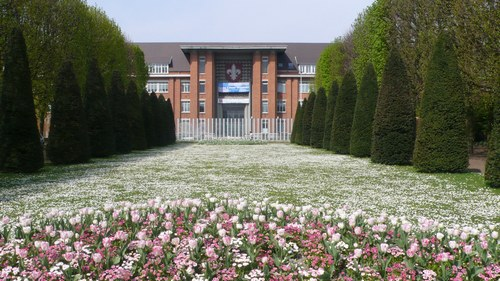
\includegraphics[height=3cm]{img/bandeau_1}
	\end{center}


	\maketitle

\end{frame}



\ifthenelse{\boolean{version_prof}}{
\begin{frame}[allowframebreaks]\titreslide{Informations professeur}
		\ifthenelse{\boolean{version_kara}}{
		\begin{bclogo}[couleur = red!70,logo=\bcpanchant]{À faire}
		\begin{itemize}
		\afaire
		\end{itemize}
		\end{bclogo}}{}

		
		\begin{bclogo}[couleur = white!30,logo=\bccalendrier]{Organisation}
		\begin{itemize}
		\organisation
		\end{itemize}
		\end{bclogo}
\end{frame}}{}
}%% Fin mode présentation
}{}%% Fin version cours

%% Version EXO

\ifthenelse{\boolean{Exo}}{
\title{Exercices}
\mode<article>{
	\lhead{\MakeUppercase{\partie}}
%    \chead{Exercice \numero}
    \rhead{Exercices}
    \lfoot{
\includegraphics[width=1.2cm]{paquets/Creative_Commons.png} \hspace{0.1cm} \etablissement - \auteur }
    \cfoot{\thepage/\pageref{LastPage}}
    \rfoot{Version \version}
    \renewcommand{\headrulewidth}{0.2pt}
    \renewcommand{\footrulewidth}{0.2pt}
    }% Fin mode article	
\mode<presentation>{
\maketitle
}
}{}%% Fin version exercice


\ifthenelse{\boolean{TD}}{
\title{TD \numero}
\mode<article>{
}% Fin mode article	
\mode<presentation>{
\maketitle
}
}{}%% Fin version TD


\section{Étude cinématique d'un robot 3 axes}
\begin{frame}\titreslide{Étude cinématique d'un robot 3 axes}
\source{Christophe Durant}
Ce TD a pour objectif de mettre en place les techniques de calcul des vecteurs vitesse et accélération d’un point
lié à un solide par rapport à un repère.\\
Nous nous intéressons pour cela au robot manipulateur de la figure 1. Ce type de robot est en particulier utilisé
dans des cellules d’assemblage (Pick and Place). Ce robot possède trois axes c'est à dire trois articulations en série
pilotées indépendamment : un axe de translation et deux axes de rotation.\\
La figure 2 constitue une première modélisation en représentant de manière simplifiée la structure du robot. La
figure 3 représente le schéma cinématique du robot.\\

DESCRIPTION DU SYSTEME :
Le robot considéré est essentiellement constitué :
\begin{itemize}
\item d’un bâti fixe 1 ;
\item d’un corps 2 qui peut se translater par rapport à 1 ;
\item d’un bras 3 mobile en rotation par rapport à 2 ;
\item d’un avant-bras 4 mobile en rotation par rapport à 3 ;
\item d’une pince (effecteur) solidaire de l' avant-bras 4.
\end{itemize}
CARACTERISTIQUES CINEMATIQUES ET GEOMETRIQUES DU SYSTEME :
\end{frame}
\begin{frame}\titreslide{Étude cinématique d'un robot 3 axes}
\question{Exprimer les coordonnées opérationnelles définissant la position $C$ dans $R_1$ en fonction des variables coordonnées articulaires $\theta_3$, $\theta_4$, $\lambda_2$ et de $L$.}
\reponse{Par relation de Chasles : $\Vecteur{O_1C}=\Vecteur{O_1A}+\Vecteur{AB}+\Vecteur{BC}=\lambda_2 \vz{1} + L \vx{3} +L\vx{4}$\\
Soit en projetant dans $R_1$...\\
On a donc : \resultat{Les 3 équations...}
}

\question{Déterminer le vecteur vitesse du point $A$ lié à $2$ par rapport à $1$}
\reponse{Par définition :
\begin{equation}\VecteurVitesse{A}{2}{1}=\DeriveeVecteur{O_1A}{R_1} \end{equation}}
\end{frame}
\end{document}